\DocumentMetadata{
  lang        = en-US,
  tagging     = on,
}

\RequirePackage{shellesc}
\documentclass[11pt, oneside]{article}   	% use "amsart" instead of "article" for AMSLaTeX format

\usepackage{geometry}                		% See geometry.pdf to learn the layout options. There are lots.
\geometry{letterpaper}                   		% ... or a4paper or a5paper or ... 
%\geometry{landscape}                		% Activate for rotated page geometry
\usepackage[parfill]{parskip}    		% Activate to begin paragraphs with an empty line rather than an indent
\usepackage{graphicx}				% Use pdf, png, jpg, or eps§ with pdflatex; use eps in DVI mode
								% TeX will automatically convert eps --> pdf in pdflatex		
\usepackage{amssymb}
\usepackage{amsmath}
\usepackage{tablefootnote}
\usepackage{multirow}
\usepackage{tabularx}
\renewcommand\tabularxcolumn[1]{m{#1}}

\usepackage{dsfont}
\usepackage[hang,flushmargin]{footmisc}
\usepackage[normalem]{ulem}

\usepackage{pgfplots,pgfplotstable}

\usepackage[autosize,forceshell]{dot2texi}
\usepackage{tikz}
\usetikzlibrary{shapes,arrows,patterns}
\usepackage{tkz-fct}

\ExplSyntaxOn
\cs_new_protected:Npn \suspendtagging #1 { \tag_suspend:n{#1} }
\cs_new_protected:Npn \resumetagging  #1 { \tag_resume:n{#1} }
\ExplSyntaxOff

\makeatletter
\long\def\ifnodedefined#1#2#3{%
    \@ifundefined{pgf@sh@ns@#1}{#3}{#2}%
}

\pgfplotsset{
    discontinuous/.style={
    scatter,
    scatter/@pre marker code/.code={
        \ifnodedefined{marker}{
            \pgfpointdiff{\pgfpointanchor{marker}{center}}%
             {\pgfpoint{0}{0}}%
             \ifdim\pgf@y>0pt
                \tikzset{options/.style={mark=*}}
                \draw [dashed,thin] (marker-|0,0) -- (0,0);
                \draw plot [mark=*,mark options={fill=white}] coordinates {(marker-|0,0)};
             \else
                \tikzset{options/.style={mark=none}}
             \fi
        }{
            \tikzset{options/.style={mark=none}}        
        }
        \coordinate (marker) at (0,0);
        \begin{scope}[options]
    },
    scatter/@post marker code/.code={\end{scope}}
    }
}

\makeatother

\newcommand*\Eval[3]{\left(#1\middle)\right\rvert_{#2}^{#3}}


\usepackage{arydshln}
\usepackage{mathtools}


%\usepackage{tagpdf}
%\tagpdfsetup{activate,paratagging,interwordspace}
\usepackage{accsupp}
\usepackage{hyperref}
\usepackage{lipsum}
%\usepackage{axessibility}
%\usepackage{accessibility}

%SetFonts
\DeclareEmphSequence{\bfseries\itshape}
\DeclareMathOperator {\ints}{\mathbb{Z}}
\DeclareMathOperator {\reals}{\mathbb{R}}
\DeclareMathOperator*{\argmin}{argmin}
\DeclareMathOperator*{\argmax}{argmax}
\DeclareMathOperator{\E}{\mathbb{E}}
\DeclareMathOperator{\V}{\mathbb{V}}


\renewcommand\labelenumi{(\theenumi)}
\renewcommand*{\thefootnote}{\fnsymbol{footnote}}

\usepackage{tcolorbox}

\newenvironment{aside}[1][Aside]{\begin{tcolorbox}[colback=black!5,colframe=black!75!black,title=#1]}{\end{tcolorbox}}


\title{Topic 20: Maximum \emph{a posteriori} Estimation}
\author{02-680: Essentials of Mathematics and Statistics}
%\date{}							% Activate to display a given date or no date

\begin{document}
\maketitle

%%%%%%%%%%%%%%%
\section{The Frequentist versus Bayesian Schools}

Both schools of statistics start with probability. 
For Bayesian inference, we take $\theta$ to be a hypothesis (the parameters) and $\mathcal{D}$ some data. 
Different people will have different a priori beliefs --- 
but we would still like to make useful inferences from data. 

When $p(\theta)$ is known, there is no disagreement, we will all just follow Bayes' Rule (Topic 14) as written. 


\begin{center}
%\suspendtagging{bayes-diagram}
\begin{dot2tex}[dot,mathmode]
digraph O {
direction="TB";
node [shape="box"];
B [label="p(\theta\mid\mathcal{D}) = \frac{p(\mathcal{D}\mid\theta)p(\theta)}{p(\mathcal{D})}"];
P [label="p(\theta\mid\mathcal{D}) = \frac{p(\mathcal{D}\mid\theta){\color{blue} p_{prior}(\theta)}}{p(\mathcal{D})}"];
F [label="\text{Likelihood }L(\theta \mid \mathcal{D}) = p(\mathcal{D}\mid\theta)"];
B->P[color="blue",label="\color{blue}\text{Bayesian}"];
B->F[color="orange",label="\color{orange}\text{Frequentist}"];
}
\end{dot2tex}
%\resumetagging{bayes-diagram}
\end{center}

When the prior is \textit{not} known, 
\emph{Bayesian} logic requires us to develop a prior based on some information we have (intuition); 
while \emph{Frequentist} logic uses only information in the provided data. 

Bayesians and frequentists take fundamentally different approaches to this challenge.
The reasons for this split are both practical (ease of implementation and computation) and 
philosophical (subjectivity versus objectivity and the nature of probability). 

The main philosophical difference concerns the \emph{meaning of probability} (recall the two perspectives from Topic 13).

%removed for tagging
%\begin{tabularx}{\textwidth}{XX}
\begin{tabular}{p{0.45\textwidth}p{0.45\textwidth}}
\hline
Bayesians & Frequentists\\
\hline\hline
the idea that probability is an abstract concept that measures a state of knowledge or a degree of belief in a given proposition &
the idea that probabilities represent long-term frequencies of repeatable random experiments\\
\hline
Subjective interpretation
& Objective interpretation\\
\hline
you ``believe'' that you will get tails 50\% of the time & 
the relative frequency of tails goes to 1/2 as the number of flips goes to infinity\\
they consider a range of values each with its own probability of being true& they consider the parameter a single fixed (if unknown) value\\
\end{tabular}

%%%%%%%%%%%%%
\section{Bayesians' Approach to Parameter Estimation}
Let's look at the coin flip example we had in the last topic: 
 $\mathcal{D} = X_1, X_2, \cdots, X_n$ 
where $X_i \sim Bernoulli(\alpha)$.
We can further summarize $\mathcal{D}$ into $c_H$ and $c_T$ 
representing the counts of heads and tails respectively. 

We saw last time that \[\hat\alpha_{MLE} = \frac{c_H}{c_H+c_T}.\]

But this is assuming we know nothing about $\alpha$ ahead of time. 
What if we \textit{believe} that it's 50/50, so we can add what are called \emph{pseudocounts}
to the input $c_{H_0}$ and $c_{T_0}$.
And thus compute 
\[\hat\alpha_{MLE-PC} = \frac{c_H+c_{H_0}}{c_H+c_T+c_{H_0}+c_{T_0}}.\]

\paragraph{Example. }
Let's assume we have an experiment where we throw a coin 100 times, we want to know $\alpha$, $c_H=0$ and $c_T=100$.

Vanilla MLE would say that 
\[\hat\alpha_{MLE} = \frac{c_H}{c_H+c_T} = \frac{0}{0 + 100} = 0\]
  
But we have a small belief this is a fair coin, so let's assume we add the pseudocounts $c_{H_0}=c_{T_0}=1$, 
in that case 
\[\hat\alpha_{MLE-PC} = \frac{c_H+c_{H_0}}{c_H+c_T+c_{H_0}+c_{T_0}}=\frac{0+1}{0+100+1+1} = \frac{1}{102}.\]

If we're more confident in our prior and set  $c_{H_0}=c_{T_0}=100$ then
\[\hat\alpha_{MLE-PC} = \frac{c_H+c_{H_0}}{c_H+c_T+c_{H_0}+c_{T_0}}=\frac{0+100}{0+100+100+100} = \frac{100}{300} = \frac{1}{3}.\]

(We will see below that these pseudocount estimates are exactly MAP estimates under a Beta prior.)

Pseudocounts are a way of exerting your \textit{belief}
\begin{itemize}
\item[] \textbf{Larger pseudocounts} – represent a strong prior belief\\\hspace*{3em}
Will have a greater effect on the posterior estimate
\item[] \textbf{Small pseudocounts} – represent a weak prior belief\\\hspace*{3em}
Will have a smaller effect on the posterior estimate
\end{itemize}

As the sample size goes to infinity, data will dominate the estimate.

\begin{aside}[An additional distribution: Beta]
The Beta distribution visually looks like an un-balanced normal. 

\begin{center}
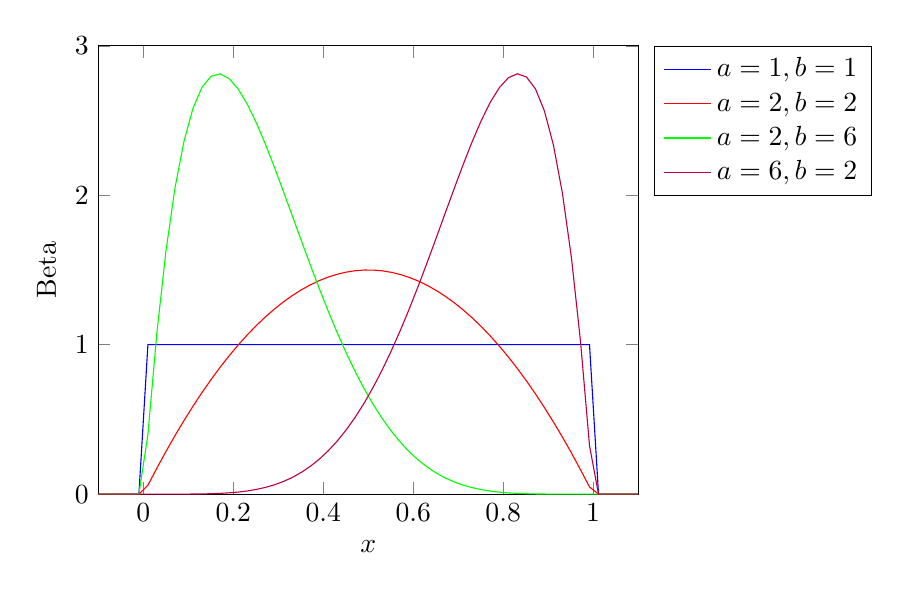
\begin{tikzpicture}[
    declare function={beta(\x,\a,\b)=\a<=0||\b<=0?1/0:\x<0||\x>1?0.0:((\x^(\a-1))*((1-\x)^(\b-1))*((\a+\b)-1)!)/((\a-1)!*(\b-1)!);}
]
\begin{axis}[
    samples=500,
    ymin=0,ymax=3,
    xmin=-0.1,xmax=1.1,
    xlabel={$x$},
    ylabel={Beta},
    legend pos=outer north east,
]
\addplot [blue] {beta(x,1,1)}; \addlegendentry{$a=1,b=1$}
\addplot [red] {beta(x,2,2)}; \addlegendentry{$a=2,b=2$}
\addplot [green] {beta(x,2,6)}; \addlegendentry{$a=2,b=6$}
\addplot [purple] {beta(x,6,2)}; \addlegendentry{$a=6,b=2$}
\end{axis}
\end{tikzpicture}
\end{center}

\[f(x;a, b) = \frac{x^{(a-1)}(1-x)^{(b-1)}}{B(a,b)}\]
where 
\[B(a,b) = \frac{\Gamma(a)\Gamma(b)}{\Gamma(a+b)}\text{ where } \Gamma(z) = (z-1)!\text{ for positive integers } z.\]
(For non-integer $z$, $\Gamma$ extends the factorial smoothly, so $a$ and $b$ need not be integers.)

When $X\sim Beta(a, b)$, $\mathbb{E}[X] = \frac{a}{a + b}$. Note $Beta(1,1)$ is the uniform distribution on $[0,1]$.

\end{aside}

We can express a prior belief about the heads probability $\alpha$ (so $\theta=(\alpha)$) with a \emph{Beta} distribution,
that is $p(\alpha)\sim Beta(a,b)$.

What is the \textit{posterior}, $p(\alpha\mid\mathcal{D})$? 
\begin{align*}
p(\alpha\mid\mathcal{D}) & = \frac{p(\mathcal{D}\mid\alpha)p(\alpha)}{p(\mathcal{D})}\\
				& \propto p(\mathcal{D}\mid\alpha)p(\alpha)\\
				& = \alpha^{c_H}(1-\alpha)^{c_T} \cdot Beta(a,b)\\
				& = \alpha^{c_H}(1-\alpha)^{c_T} \cdot \frac{\alpha^{(a-1)}(1-\alpha)^{(b-1)}}{B(a,b)}\\
				& \propto \alpha^{(c_H+a-1)}(1-\alpha)^{(c_T+b-1)}
\end{align*}
which is the density of a $Beta(c_H+a,\ c_T+b)$ distribution.
(As in Topic 19 we used the likelihood of the observed sequence. If we only recorded the counts, a binomial coefficient would appear, 
but it is constant in $\alpha$ and drops out.)

\paragraph{Connection to pseudocounts.} The mean of a $Beta(c_H+a,\ c_T+b)$ distribution is $\frac{c_H+a}{c_H+c_T+a+b}$, 
so the pseudocount estimate from above with $c_{H_0}=a$ and $c_{T_0}=b$ is the posterior \emph{mean}. 
MAP instead uses the posterior \emph{mode}, which we derive in the example on unknown priors below.

%%%%%%%%%%%%%
\section{Maximum \textit{a Posteriori} (MAP) Estimation}

As a reminder 
\[\hat\theta_{MLE} = \argmax_{\theta\in\Theta} p(\mathcal{D}\mid \theta).\]
On the other hand if we want to include information of our prior knowledge 
then we have MAP:
\[\hat\theta_{MAP} = \argmax_{\theta\in\Theta} p(\theta\mid\mathcal{D}) =  \argmax_{\theta\in\Theta} p(\mathcal{D}\mid \theta)\cdot p(\theta).\]

Note that in both cases we're making a \emph{point estimate} of $\theta$. 
We still don't have the whole picture, we're using data to estimate our model, 
but MAP is \emph{partially Bayesian}.

If the prior is flat (uniform), $p(\theta)$ is constant and does not change the $\argmax$, so MAP gives the same answer as MLE. 
That is why we could ignore $p(\theta)$ in Topic 19. A prior that is not flat, such as the pseudocounts above, pulls the estimate toward our prior belief. 


%%%%%%%%%%%%%%%
\subsection{Example: \textit{Known} Prior}
There are three types of coins which have different probabilities of landing heads when tossed
\begin{itemize}
\item[] Type $A$ coins are fair and have probability 0.5 of heads
\item[] Type $B$ coins are bent and have probability 0.6 of heads
\item[] Type $C$ coins are bent and have probability 0.9 of heads
\end{itemize}

Suppose you have a drawer containing 10 coins: 
5 of type $A$, 3 of type $B$, and 2 of type $C$. 
You reach into the drawer and pick a coin at random. 
Without showing you the coin, it is flipped \textbf{once} and lands \textbf{tails}. 
What is the probability it is type $A$? Type $B$? Type $C$? 

\begin{center}
\begin{tabular}{|c||c|c|c|c|}
\hline
Hypothesis & Prior & Likelihood & Bayes Numerator & Posterior\\
$\theta$ & $p(\theta)$ & $p(\mathcal{D}\mid\theta)$ & $p(\mathcal{D}\mid\theta)\cdot p(\theta)$ & $p(\theta\mid\mathcal{D})$\\
\hline
\hline
$A$	& 0.5		& 0.5		& 0.25	& $\approx0.641$\\
$B$	& 0.3		& 0.4		& 0.12	& $\approx0.308$\\
$C$	& 0.2		& 0.1		& 0.02	& $\approx0.051$\\
\hline
\end{tabular}
\end{center}

Thus $\hat\theta_{MAP} = A$. 

What if you then flip the same coin another 9 times, so including the first coin we have 
$c_H=6$ and $c_T=4$.
Notice in the table below, the prior does not change. 

\begin{center}
\begin{tabular}{|c||c|c|c|c|}
\hline
Hypothesis & Prior & Likelihood & Bayes Numerator & Posterior\\
$\theta$ & $p(\theta)$ & $p(\mathcal{D}\mid\theta)$ & $p(\mathcal{D}\mid\theta)\cdot p(\theta)$ & $p(\theta\mid\mathcal{D})$\\
\hline
\hline
$A$	& 0.5		& $0.98\times10^{-3}$ & $4.88\times10^{-4}$	& 0.570\\
$B$	& 0.3		& $1.19\times10^{-3}$ & $3.58\times10^{-4}$	& 0.418\\
$C$	& 0.2		& $0.05\times10^{-3}$ & $0.11\times10^{-4}$	& 0.012\\
\hline
\end{tabular}
\end{center}

In this case, it's still true that $\hat\theta_{MAP} = A$,
but $\hat\theta_{MLE} = B$. 


%%%%%%%%%%%%%%%
\subsection{\textit{Unknown} Prior}
Assume we have a similar scenario but this time there is no list of hypotheses with known prior probabilities (as in the coin drawer). 
Instead we choose a prior \emph{distribution} for the parameter (see conjugate priors below), 
and follow a similar procedure to that for MLE: 
take the zero point of the log of the posterior. 
\[\frac{d}{d\theta} \ln\bigl[p(\mathcal{D}\mid\theta)\,p(\theta)\bigr] = 0\]

\paragraph{Example: Bernoulli with a Beta prior.}
Let $X_i\sim Bernoulli(\alpha)$ with $c_H$ heads and $c_T$ tails, and a prior $\alpha\sim Beta(a,b)$. 
From above, the posterior is proportional to $\alpha^{(c_H+a-1)}(1-\alpha)^{(c_T+b-1)}$. 
Following the recipe from Topic 19, take the log and find the zero of the derivative:
\begin{align*}
\frac{d}{d\alpha} \ln\left[\alpha^{(c_H+a-1)}(1-\alpha)^{(c_T+b-1)}\right]
& = \frac{d}{d\alpha}\left[(c_H+a-1)\ln\alpha + (c_T+b-1)\ln(1-\alpha)\right]\\
& = \frac{c_H+a-1}{\alpha} - \frac{c_T+b-1}{1-\alpha} = 0.
\end{align*}
Solving gives
\[\hat\alpha_{MAP} = \frac{c_H+a-1}{c_H+c_T+a+b-2}.\]
This is the Bernoulli MLE from Topic 19 with $a-1$ extra heads and $b-1$ extra tails, 
so it is exactly the pseudocount estimate from above with pseudocounts $c_{H_0}=a-1$ and $c_{T_0}=b-1$. 
For the coin with $c_H=0$ and $c_T=100$: a $Beta(2,2)$ prior (pseudocounts of $1$) gives $\hat\alpha_{MAP}=\frac{1}{102}$, 
while the flat $Beta(1,1)$ prior gives $\hat\alpha_{MAP}=0$, the same as the MLE.

\begin{aside}[Conjugate Priors]
Definition: If the prior and the posterior belong to the same parametric family, 
then the prior is said to be conjugate for the likelihood.
Parameters of the prior distribution
are often called ``hyperparameters''.\\
Example: $a,b$ in $Beta(a,b)$.
\vspace{1em}

How do you set the hyperparameters?
\begin{itemize}
\item Prior knowledge (from experienced domain-specific experts)
\item If no prior knowledge, use “uninformative” prior (e.g., $Beta(1,1)$, which is flat, so MAP equals MLE)
\end{itemize}
\vspace{1em}

Some common conjugate prior sets are in the table below:
\begin{center}\begin{tabular}{|c|c|c|}
\hline
Prior & Likelihood & Posterior\\
\hline\hline
Beta & Bernoulli & Beta\\
Beta & Binomial & Beta\\
Gamma & Poisson & Gamma\\
Normal & Normal & Normal\\
\hline
\end{tabular}\end{center}

The Bernoulli, Normal, and Poisson likelihoods are the ones whose MLEs we derived in Topic 19. 
(We do not define the Gamma distribution here; it is the standard prior for a Poisson rate $\lambda$.)

\end{aside}

\section*{Useful References}
Wasserman. ``All of Statistics: A Concise Course in Statistical Inference'' \S11
Degroot and Schervish. ``Probability and Statistics''  \S\S7.1-7.4


\end{document}